\documentclass[11pt]{standalone}
\usepackage{tikz}
\usepackage{pgfplots}
\pgfplotsset{compat=1.15}
\usetikzlibrary{shapes.geometric}
\usetikzlibrary{arrows.meta,calc,decorations.pathmorphing,shapes.geometric,backgrounds,plotmarks,shapes.multipart,calc}
\begin{document} 
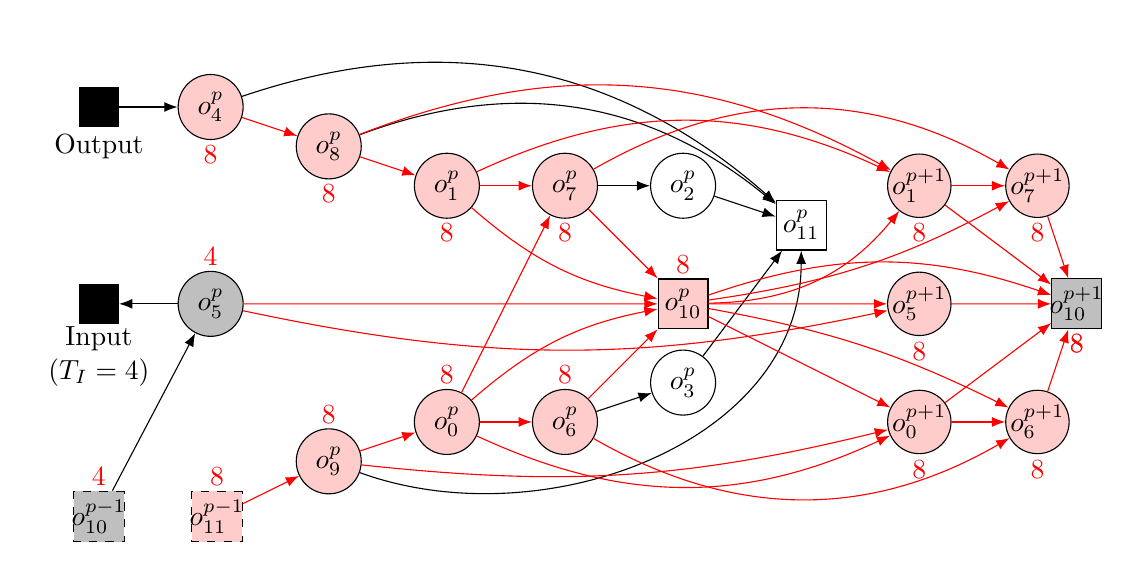
\begin{tikzpicture}

\begin{scope}[framed,local bounding box=scope1,node distance=1.5cm,every node/.style={circle,draw},square/.style={regular polygon,regular polygon sides=4,inner sep=-.3},invisible/.style={minimum width=0mm,inner sep=0mm,outer sep=0mm,draw=none}]
% Nodes
\node[fill=gray!50] (o5) {$o_5^p$};
\node[above of = o5,yshift=1cm,fill=red!20] (o4) {$o_4^p$};
\node[right of = o4,yshift=-.5cm,fill=red!20] (o8) {$o_8^p$};
\node[right of = o8,yshift=-.5cm,fill=red!20] (o1) {$o_1^p$};
\node[right of = o1,fill=red!20] (o7) {$o_7^p$};
\node[right of = o7] (o2) {$o_2^p$};
\node[square,right of = o2,yshift=-.5cm] (o11) {$o_{11}^p$};
\node[square,below of = o2,fill=red!20] (o10) {$o_{10}^p$};
\node[below of = o10,yshift=.5cm] (o3) {$o_3^p$};
\node[left of = o3,yshift=-.5cm,fill=red!20] (o6) {$o_6^p$};
\node[left of = o6,fill=red!20] (o0) {$o_0^p$};
\node[left of = o0,yshift=-.5cm,fill=red!20] (o9) {$o_9^p$};

\node[right of = o11,yshift=.5cm,inner sep=0,fill=red!20] (o1_1) {$o_1^{p+1}$};
\node[below of = o1_1,inner sep=0,fill=red!20] (o5_1) {$o_5^{p+1}$};
\node[below of = o5_1,inner sep=0,fill=red!20] (o0_1) {$o_0^{p+1}$};
\node[right of = o1_1,inner sep=0,fill=red!20] (o7_1) {$o_7^{p+1}$};
\node[right of = o0_1,inner sep=0,fill=red!20] (o6_1) {$o_6^{p+1}$};
\node[regular polygon,regular polygon sides=4,inner sep=-3.4,right of = o5_1,xshift=.5cm,fill=gray!50] (o10_1) {$o_{10}^{p+1}$};

\node[draw=none,below of = o10_1,yshift=1cm,text=red] {$8$};

\node[draw=none,below of = o4,yshift=.9cm,text=red] {$8$};
\node[draw=none,below of = o8,yshift=.9cm,text=red] {$8$};
\node[draw=none,below of = o1,yshift=.9cm,text=red] {$8$};
\node[draw=none,below of = o7,yshift=.9cm,text=red] {$8$};
\node[draw=none,above of = o10,yshift=-1cm,text=red] {$8$};
\node[draw=none,below of = o1_1,yshift=.9cm,text=red] {$8$};
\node[draw=none,below of = o5_1,yshift=.9cm,text=red] {$8$};
\node[draw=none,below of = o0_1,yshift=.9cm,text=red] {$8$};
\node[draw=none,below of = o6_1,yshift=.9cm,text=red] {$8$};
\node[draw=none,below of = o7_1,yshift=.9cm,text=red] {$8$};
\node[draw=none,below of = o10_1,yshift=1cm,text=red] {$8$};
\node[draw=none,above of = o6,yshift=-.9cm,text=red] {$8$};
\node[draw=none,above of = o0,yshift=-.9cm,text=red] {$8$};
\node[draw=none,above of = o9,yshift=-.9cm,text=red] {$8$};

%arcs
\path (o5) edge[-{Latex[]},red] (o10);
\path (o4) edge[-{Latex[]},red] (o8);
\path (o4) edge[-{Latex[]},bend left=30] (o11);
\path (o8) edge[-{Latex[]},red] (o1);
\path (o8) edge[-{Latex[]},bend left=30] (o11);
\path (o1) edge[-{Latex[]},red] (o7);
\path (o1) edge[-{Latex[]},bend right=15,red] (o10);
\path (o7) edge[-{Latex[]}] (o2);
\path (o7) edge[-{Latex[]},red] (o10);
\path (o2) edge[-{Latex[]}]  (o11);
\path (o9) edge[-{Latex[]},red]  (o0);
\path (o9) edge[-{Latex[]}, out=340,in=270]  (o11);
\path (o0) edge[-{Latex[]},red]  (o6);
\path (o0) edge[-{Latex[]},bend left=15,red]  (o10);
\path (o6) edge[-{Latex[]}]  (o3);
\path (o6) edge[-{Latex[]},red]  (o10);
\path (o3) edge[-{Latex[]}]  (o11);
\path (o0) edge[-{Latex[]},red]  (o7);

\path (o5_1) edge[-{Latex[]},red]  (o10_1);
\path (o6_1) edge[-{Latex[]},red]  (o10_1);
\path (o7_1) edge[-{Latex[]},red]  (o10_1);
\path (o0_1) edge[-{Latex[]},red]  (o10_1);
\path (o1_1) edge[-{Latex[]},red]  (o10_1);

\path (o10) edge[-{Latex[]},bend right = 25,red]  (o1_1);
\path (o1) edge[-{Latex[]},bend left = 25,red]  (o1_1);
\path (o8) edge[-{Latex[]},bend left = 25,red]  (o1_1);

\path (o10) edge[-{Latex[]},red]  (o5_1);
\path (o5) edge[-{Latex[]},bend right = 12,red]  (o5_1);

\path (o10) edge[-{Latex[]},red]  (o0_1);
\path (o0) edge[-{Latex[]},bend right = 25,red]  (o0_1);
\path (o9) edge[-{Latex[]},bend right = 10,red]  (o0_1);

\path (o10) edge[-{Latex[]},bend right = 10,red]  (o7_1);
\path (o1_1) edge[-{Latex[]},red]  (o7_1);
\path (o7) edge[-{Latex[]},bend left = 30,red]  (o7_1);

\path (o10) edge[-{Latex[]},bend left = 8,red]  (o6_1);
\path (o0_1) edge[-{Latex[]},red]  (o6_1);
\path (o6) edge[-{Latex[]},bend right = 30,red]  (o6_1);

\path (o10) edge[-{Latex[]},bend left = 19,red]  (o10_1);

\node[rectangle,draw,fill=black,minimum height=.5cm, minimum width=.5cm,xshift=-1cm,label={[align=center,yshift=.5cm]south:Input\\($T_I = 4$)}] at(o5.west) (input){};

\path (input) edge[{Latex[]}-]  (o5);

\node[rectangle,draw,fill=black,minimum height=.5cm, minimum width=.5cm,xshift=-1cm,label={[align=center,yshift=.5cm]south:Output}] at(o4.west) (output){};

\path (output) edge[-{Latex[]}]  (o4);


\node (c1) [invisible] at ([xshift=.2cm,yshift=-1.2cm]o10_1){};
\node (c2) [invisible] at ([yshift=-1.2cm]o0_1){};


\node[regular polygon,regular polygon sides=4,inner sep=-3.4,dashed,fill=gray!50] at(input |- c2) (o10_0) {$o_{10}^{p-1}$};
\path (o10_0) edge[-{Latex[]}]  (o5);

\node[regular polygon,regular polygon sides=4,inner sep=-3.4,right of = o10_0,dashed,fill=red!20]  (o11_0) {$o_{11}^{p-1}$};
\path (o11_0) edge[-{Latex[]},red]  (o9);

\node[draw=none,above of = o5,yshift=-.9cm,text=red] {$4$};
\node[draw=none,above of = o10_0,yshift=-1cm,text=red] {$4$};
\node[draw=none,above of = o11_0,yshift=-1cm,text=red] {$8$};



\end{scope}

\end{tikzpicture}
\end{document}